% Overleaf/LaTeX assets for HCI Bimodal Affective Alignment (class project)
% This content is designed for IEEEtran and can be copied into the main manuscript.

\subsection{System Architecture}
The implemented pipeline combines text emotion inference (\texttt{app/text\_emotion.py}) and face emotion inference (\texttt{app/face\_emotion.py}) into a weighted fusion layer (\texttt{app/fusion.py}). The fused emotion drives empathetic response generation in \texttt{app/response\_generator.py}. The architecture is intentionally deterministic and reproducible for classroom evaluation and reporting.

\begin{figure}[t]
    \centering
    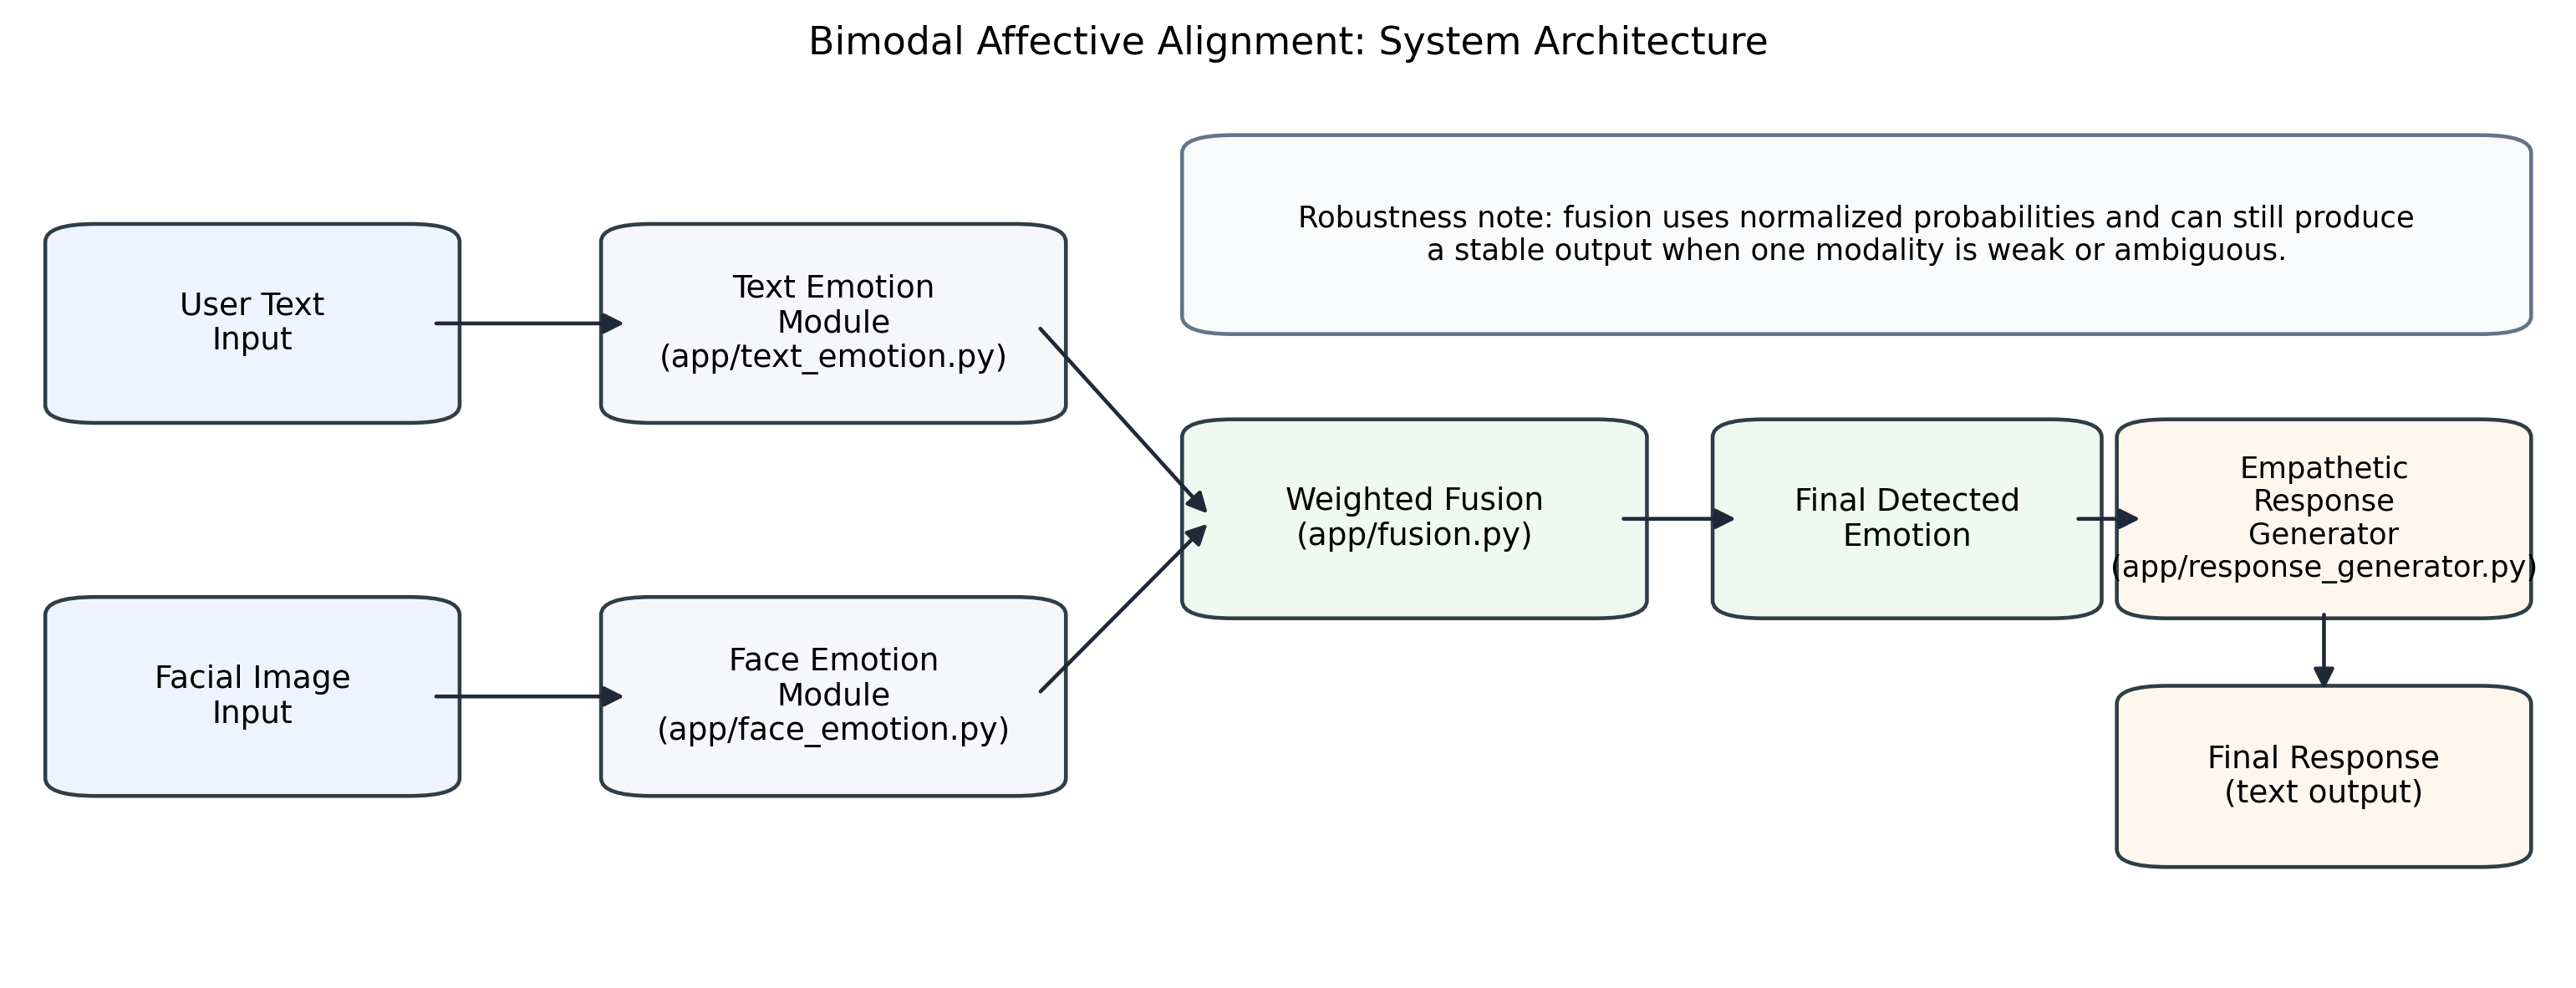
\includegraphics[width=\linewidth]{figures/system_architecture.png}
    \caption{Bimodal system architecture with text and facial streams, weighted fusion, and response generation.}
    \label{fig:system_architecture}
\end{figure}

\begin{figure}[t]
    \centering
    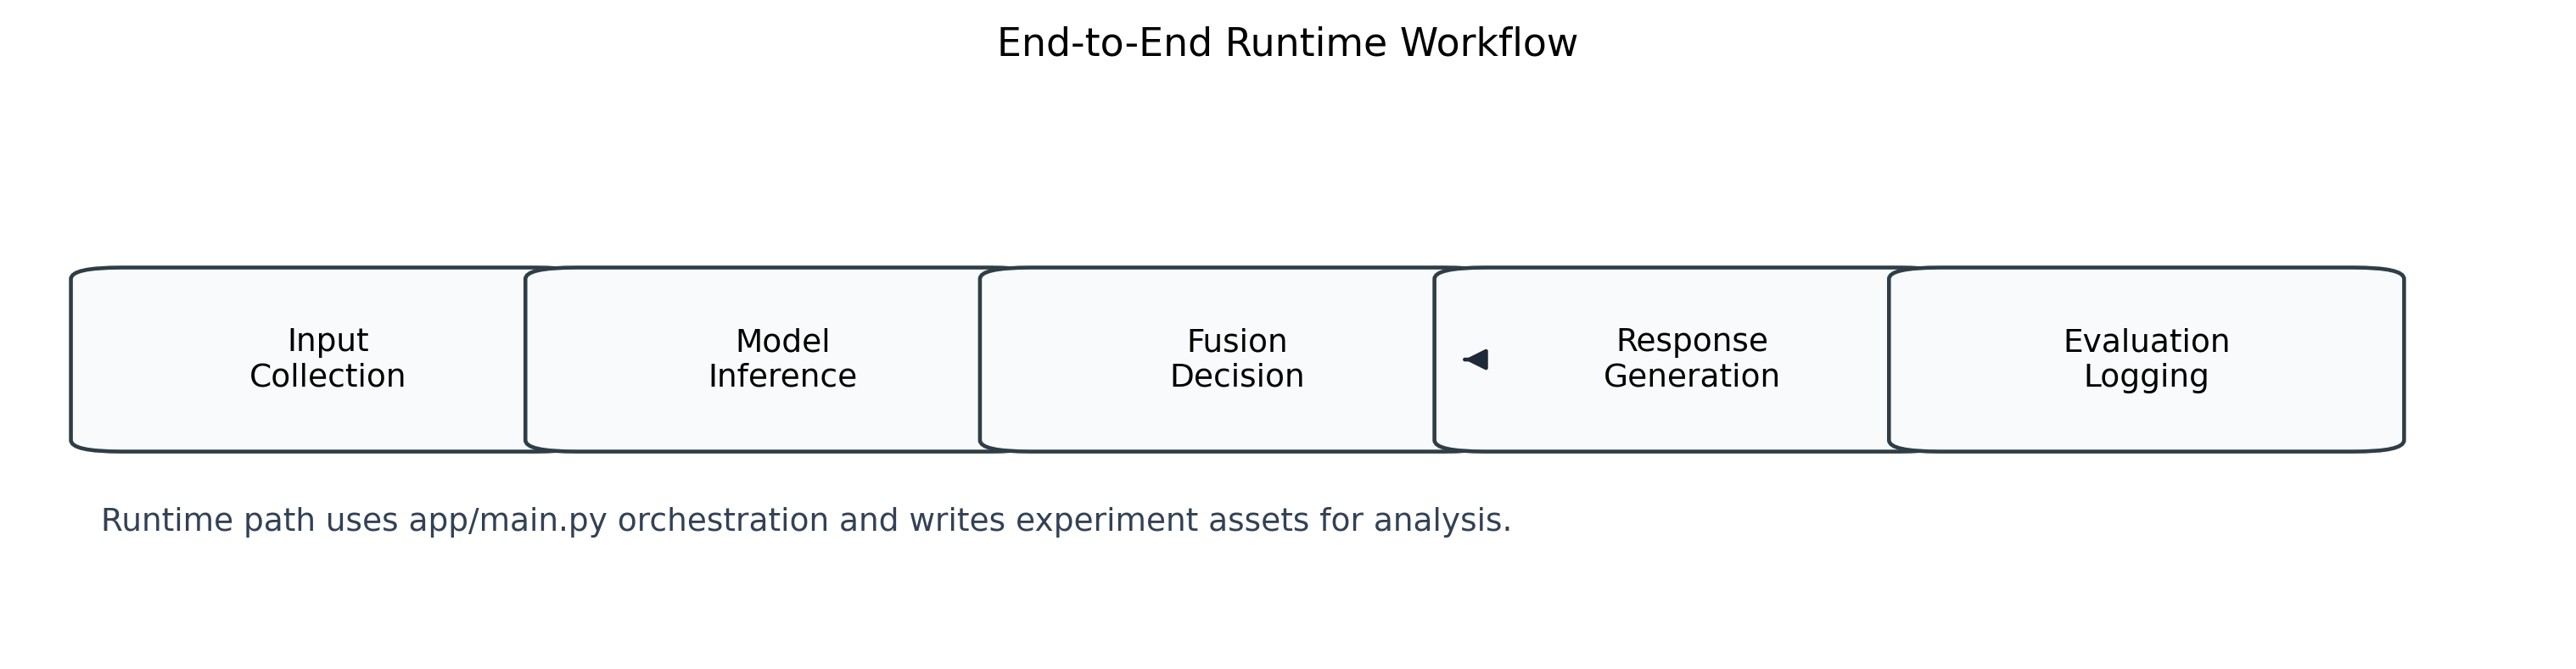
\includegraphics[width=\linewidth]{figures/runtime_workflow.png}
    \caption{Operational runtime workflow from input collection to evaluation logging.}
    \label{fig:runtime_workflow}
\end{figure}

\subsection{Fusion Strategy}
The project uses a convex combination of modality-level probabilities:
\begin{equation}
P_{fusion}(e)=\alpha P_{text}(e)+(1-\alpha)P_{face}(e), \quad \hat{e}=\arg\max_e P_{fusion}(e)
\label{eq:fusion_rule}
\end{equation}
where $\alpha\in[0,1]$ controls modality emphasis. In this classroom prototype, alpha sensitivity is evaluated via a sweep over $\{0.0,0.25,0.5,0.75,1.0\}$.

\begin{figure}[t]
    \centering
    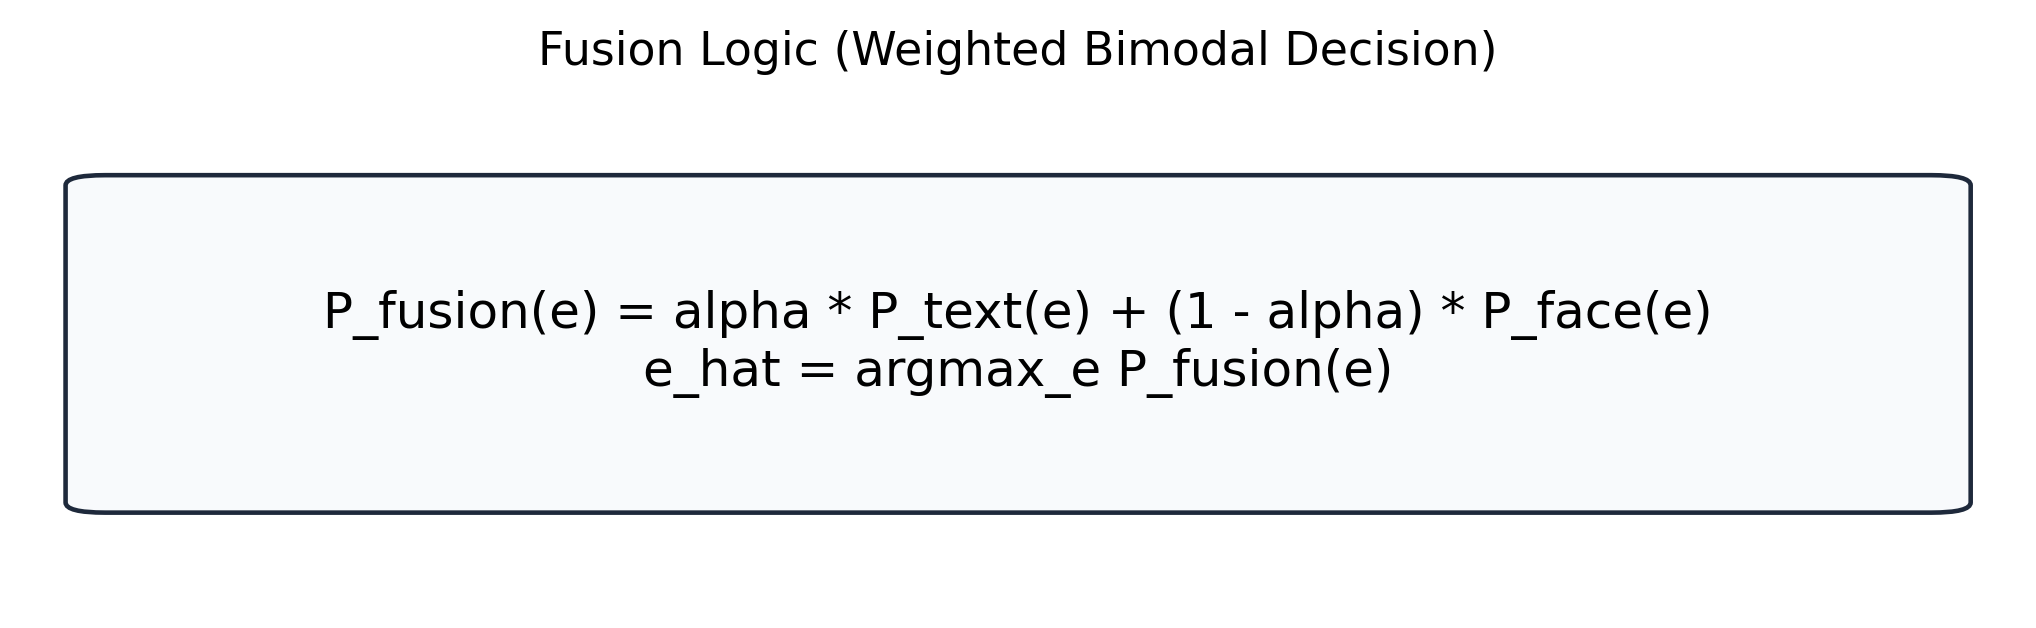
\includegraphics[width=0.95\linewidth]{figures/fusion_equation.png}
    \caption{Weighted fusion rule used in the implemented bimodal decision layer.}
    \label{fig:fusion_equation}
\end{figure}

\subsection{Evaluation Setup}
Evaluation combines automatic outputs and a human-rating workflow. Automatic artifacts include ablation and alpha-sensitivity plots generated from \texttt{experiments/*.csv}. Human evaluation uses a structured rating sheet and aggregation utility in \texttt{app/final\_evaluation\_pack.py}. Current human results are \textbf{preliminary}: pilot data from one completed rater (R1).

\begin{figure}[t]
    \centering
    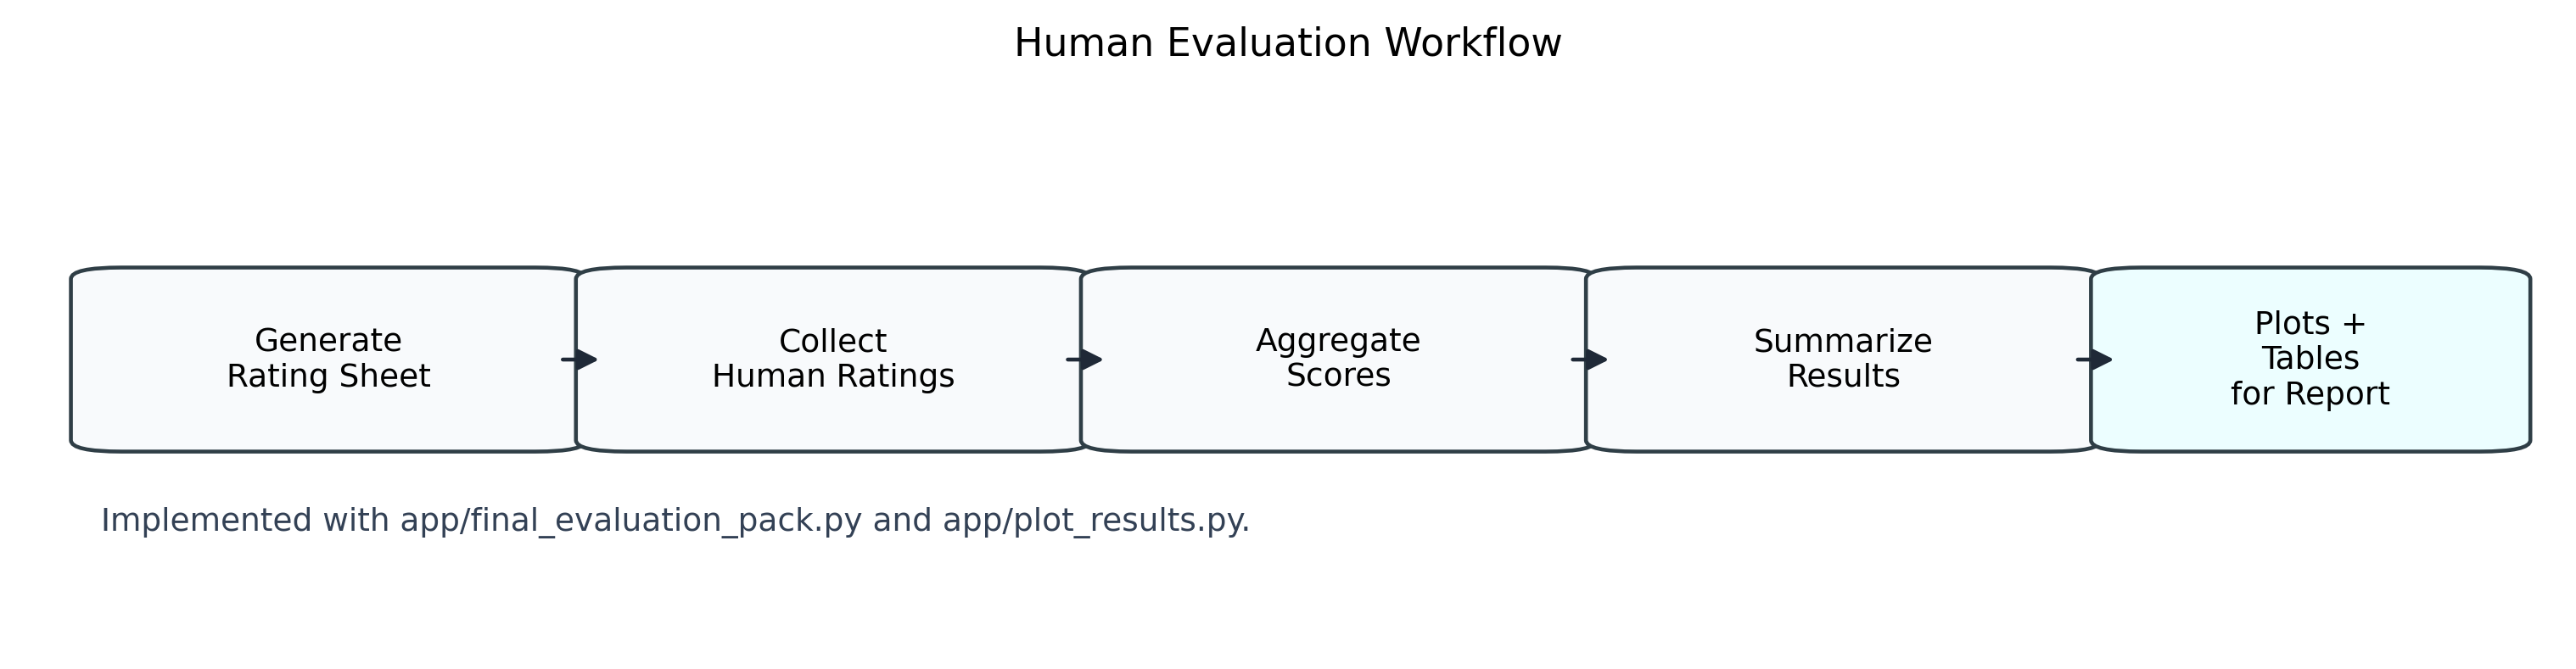
\includegraphics[width=\linewidth]{figures/human_eval_workflow.png}
    \caption{Human evaluation workflow from rating-sheet generation to aggregated summaries.}
    \label{fig:human_eval_workflow}
\end{figure}

\begin{figure}[t]
    \centering
    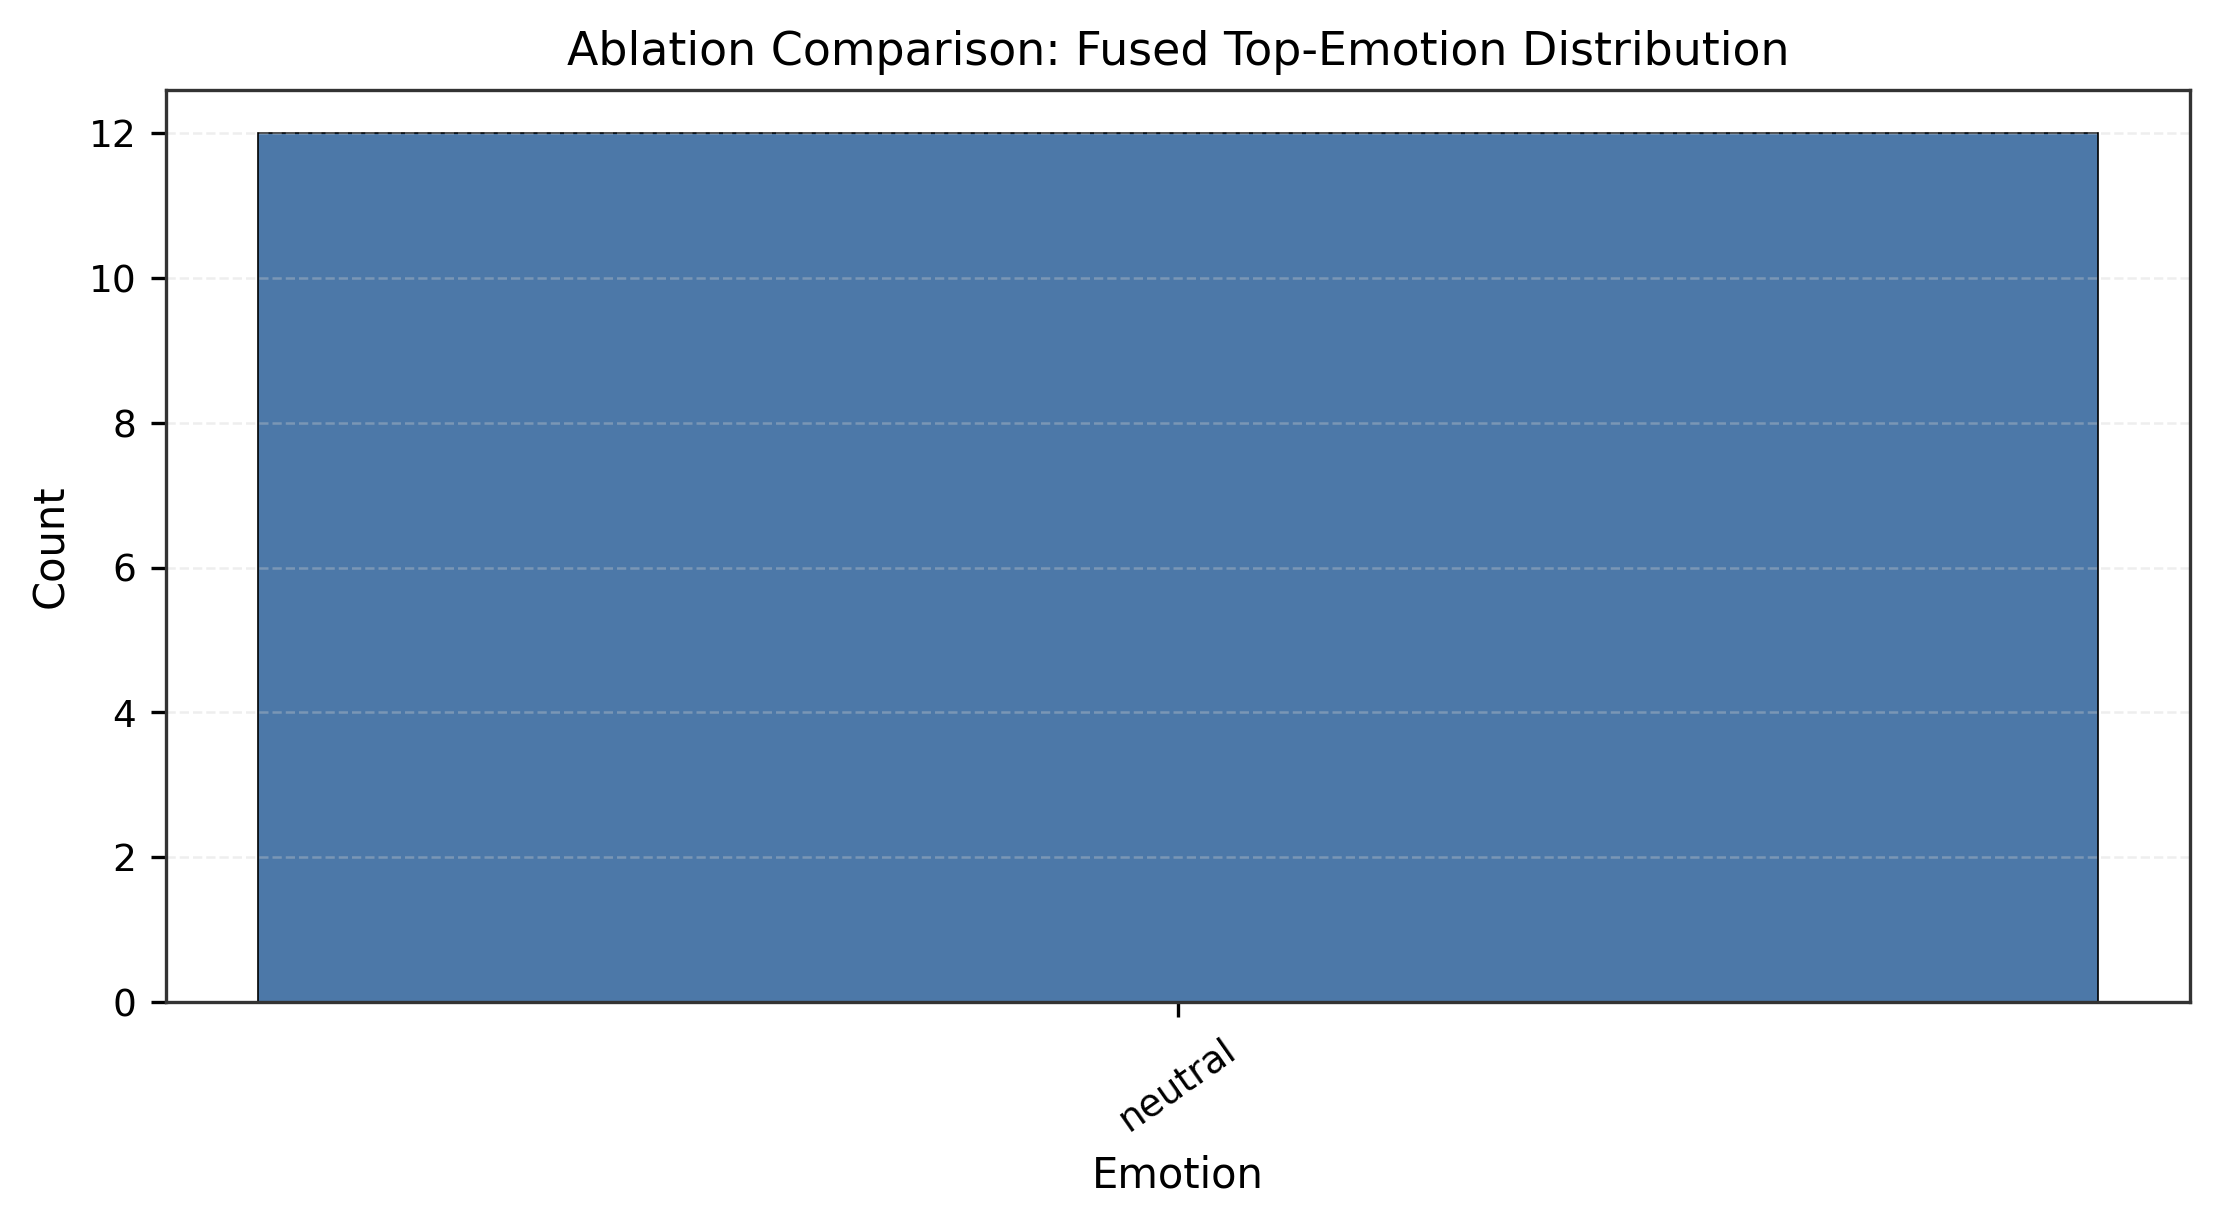
\includegraphics[width=\linewidth]{figures/ablation_comparison_plot.png}
    \caption{Ablation comparison using fused top-emotion counts.}
    \label{fig:ablation_plot}
\end{figure}

\begin{figure}[t]
    \centering
    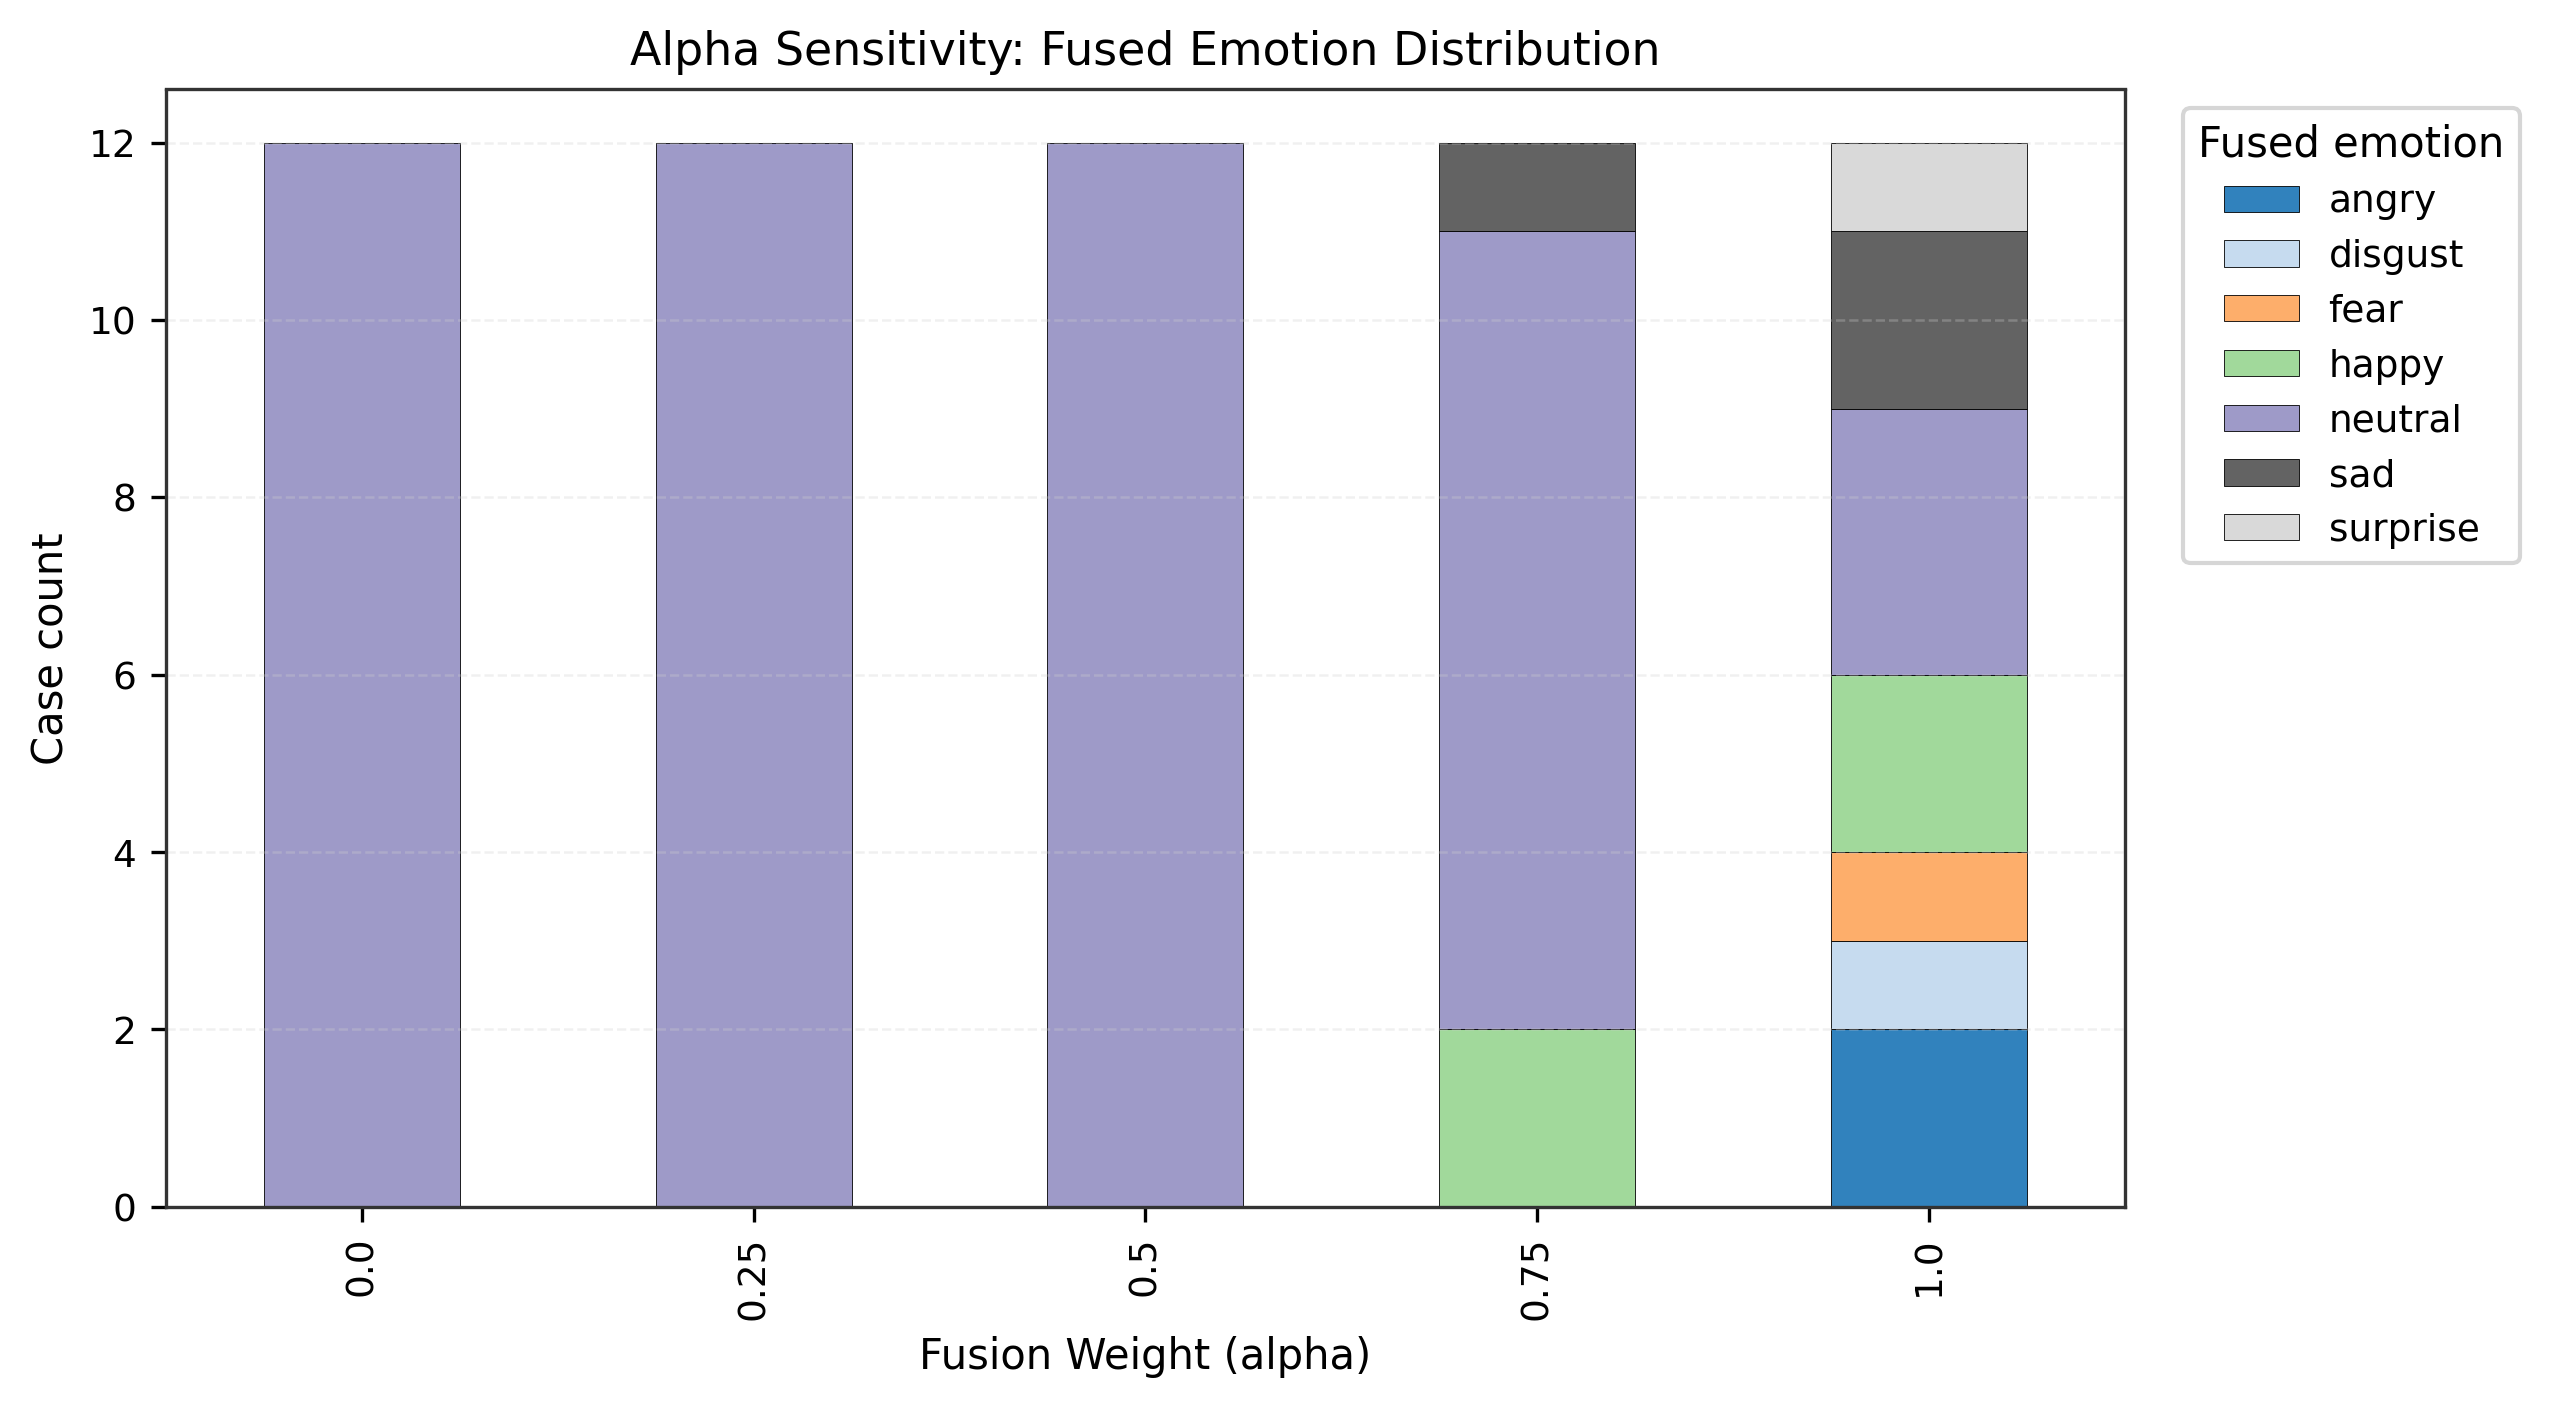
\includegraphics[width=\linewidth]{figures/alpha_sensitivity_plot.png}
    \caption{Alpha sensitivity across the implemented fusion sweep.}
    \label{fig:alpha_sensitivity_plot}
\end{figure}

\begin{figure}[t]
    \centering
    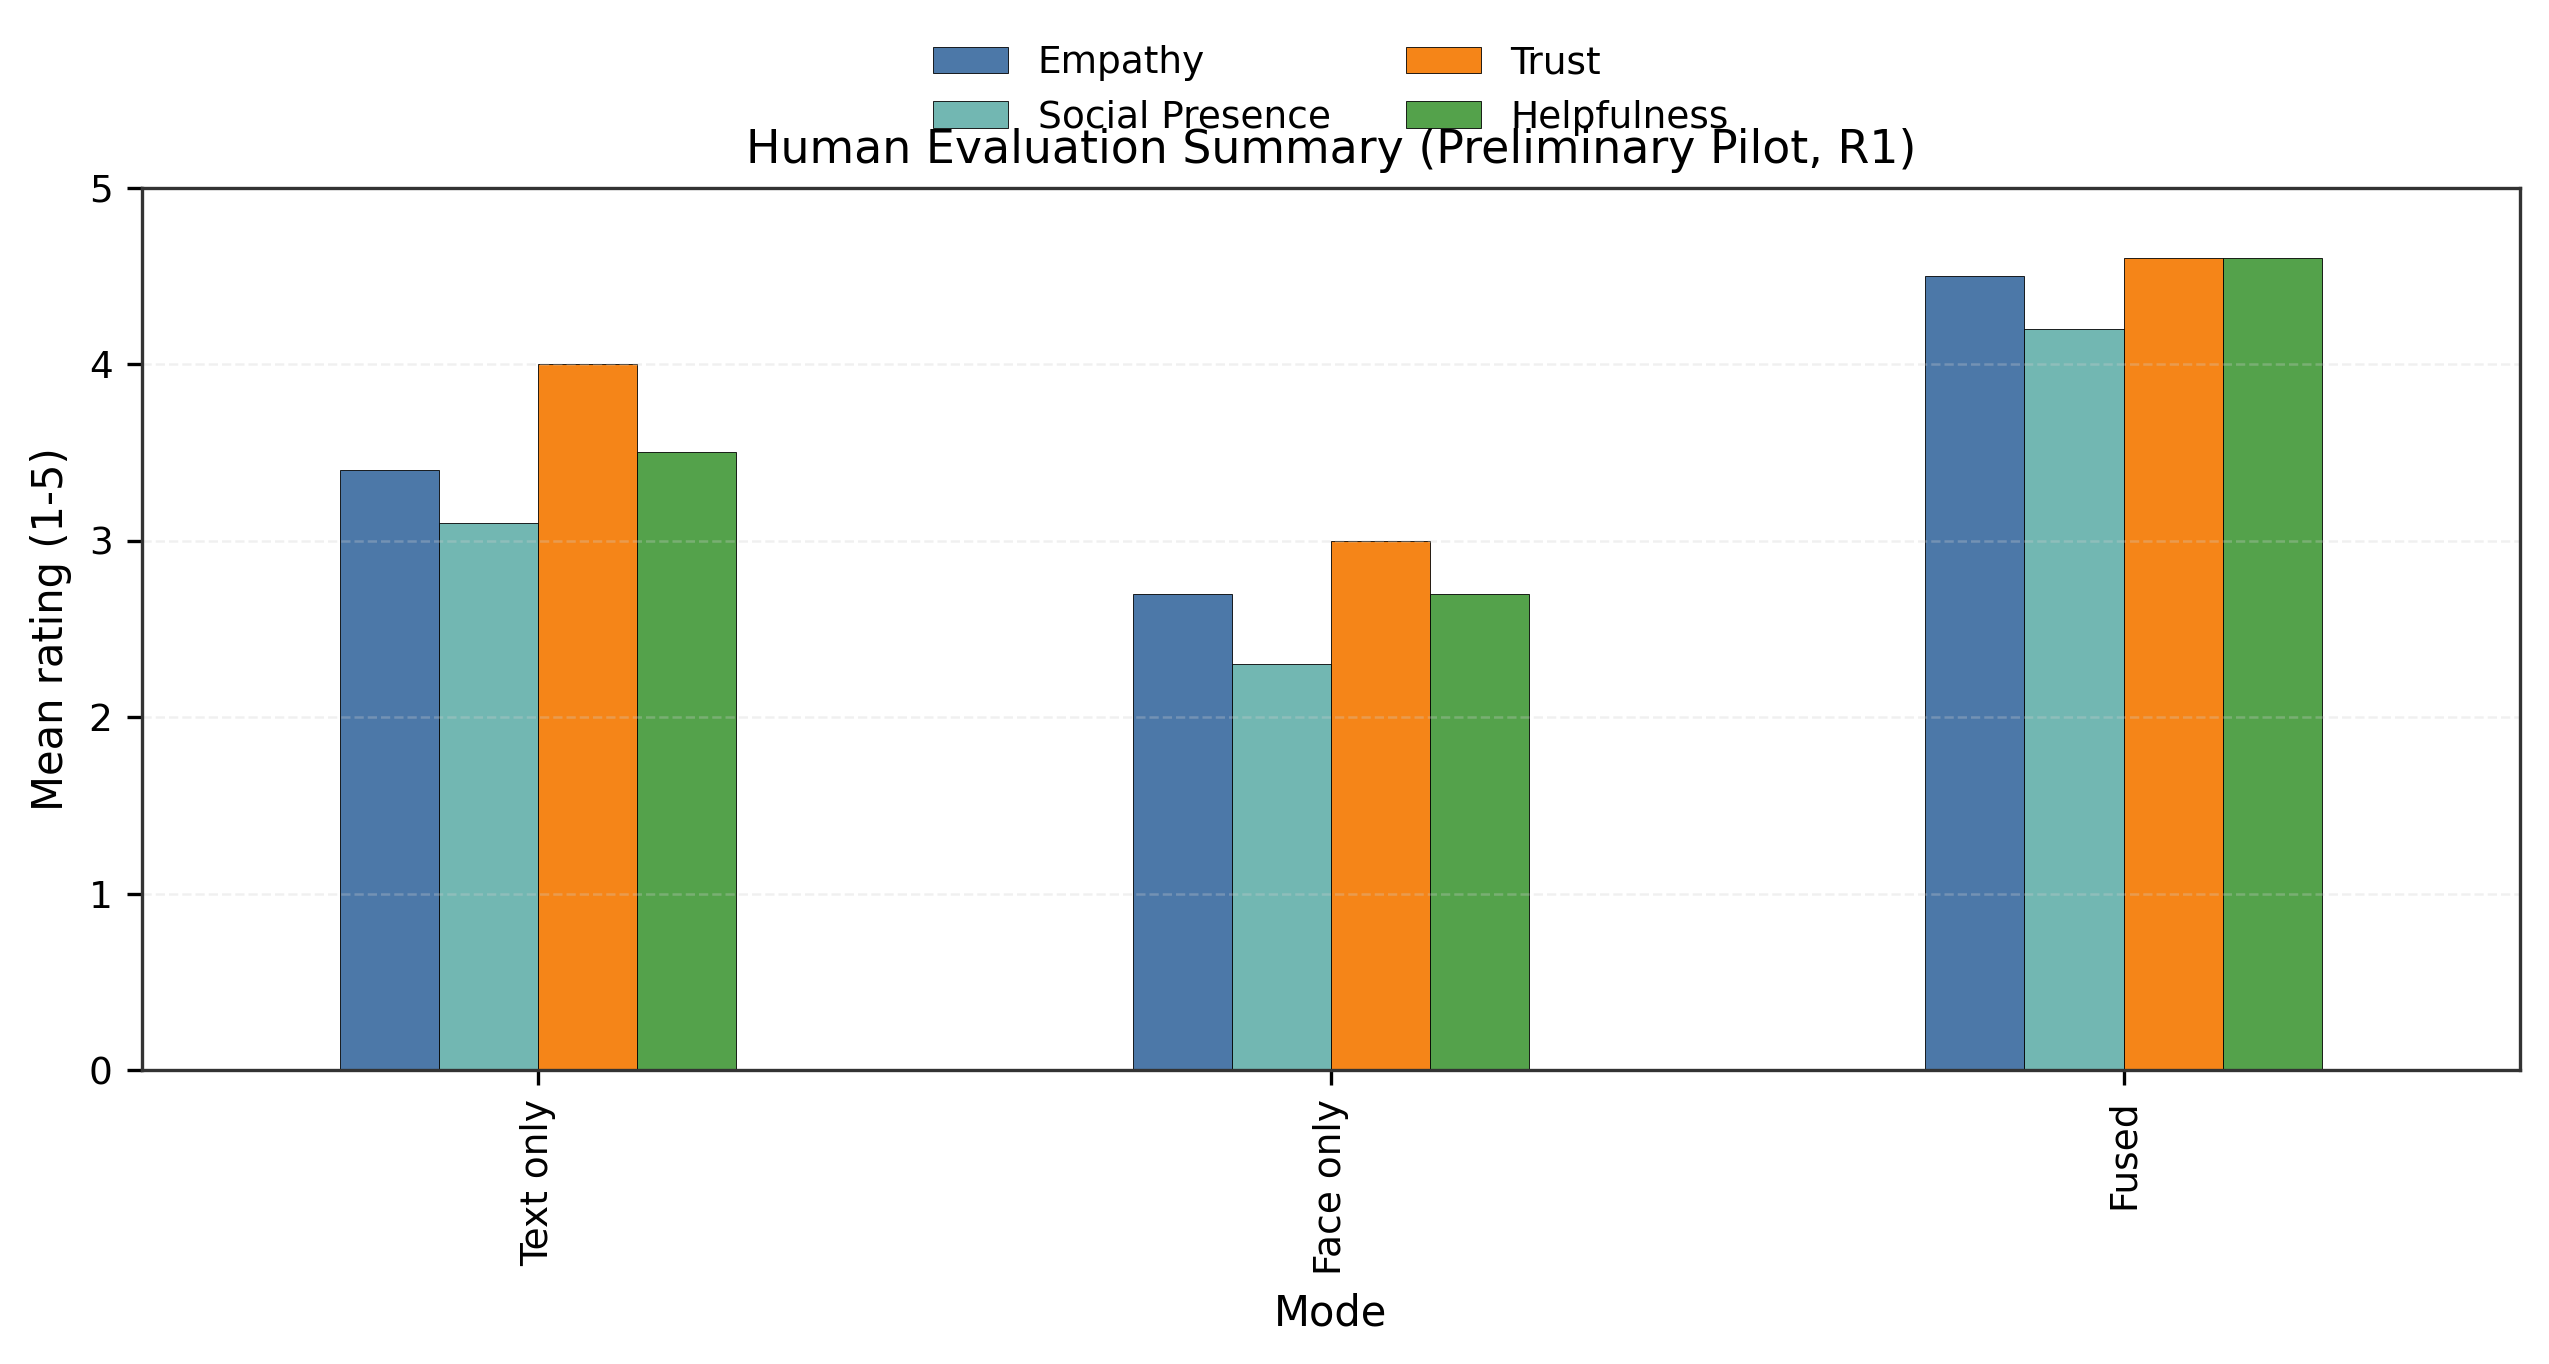
\includegraphics[width=\linewidth]{figures/human_eval_summary_plot.png}
    \caption{Preliminary pilot human evaluation summary (one completed rater, R1).}
    \label{fig:human_eval_summary_plot}
\end{figure}

\begin{figure}[t]
    \centering
    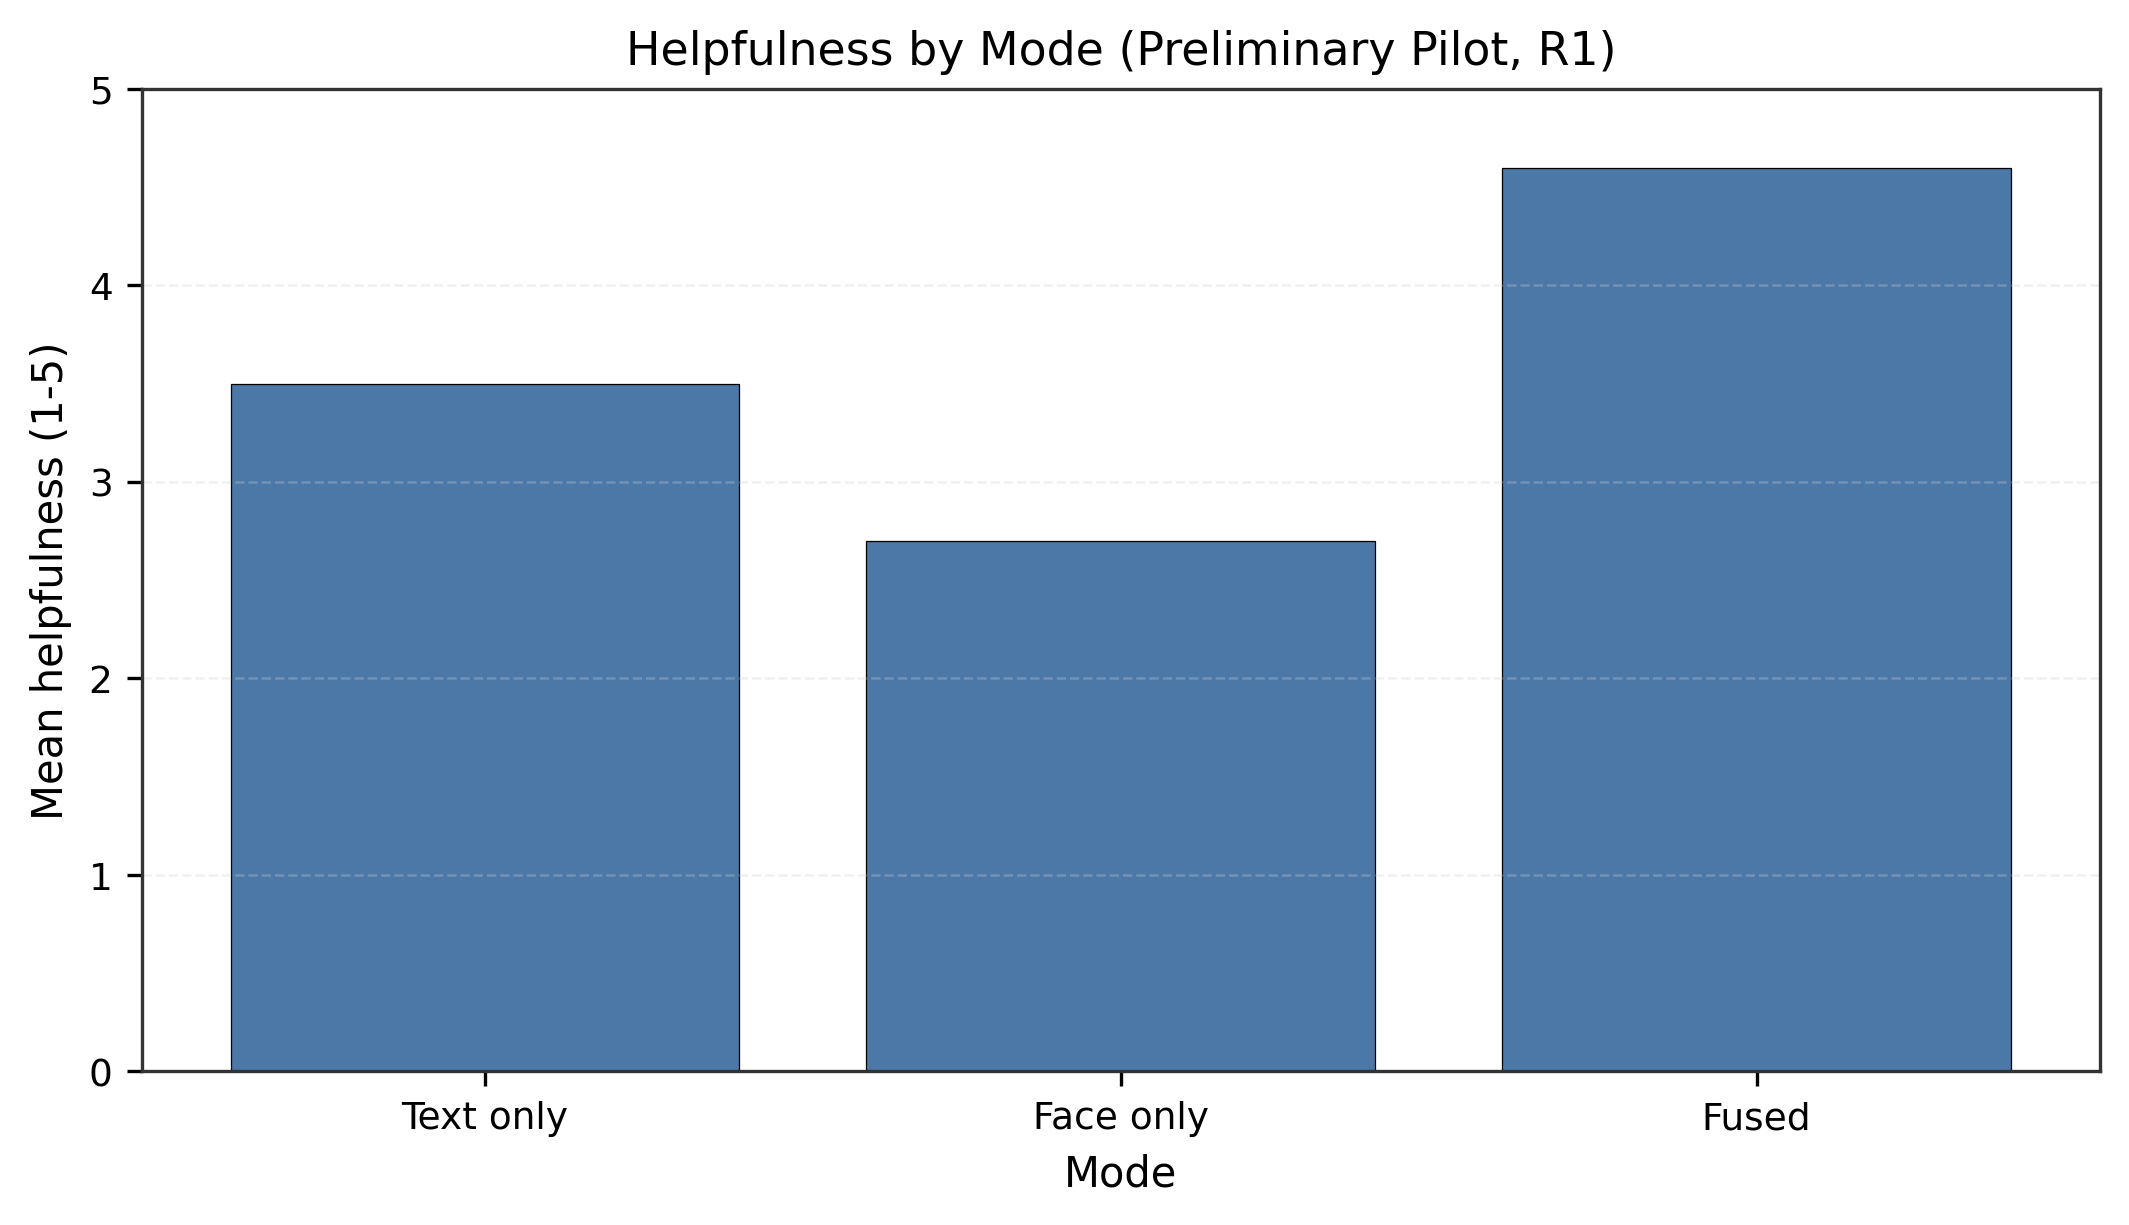
\includegraphics[width=\linewidth]{figures/helpfulness_plot.png}
    \caption{Pilot helpfulness means by mode.}
    \label{fig:helpfulness_plot}
\end{figure}

\begin{figure}[t]
    \centering
    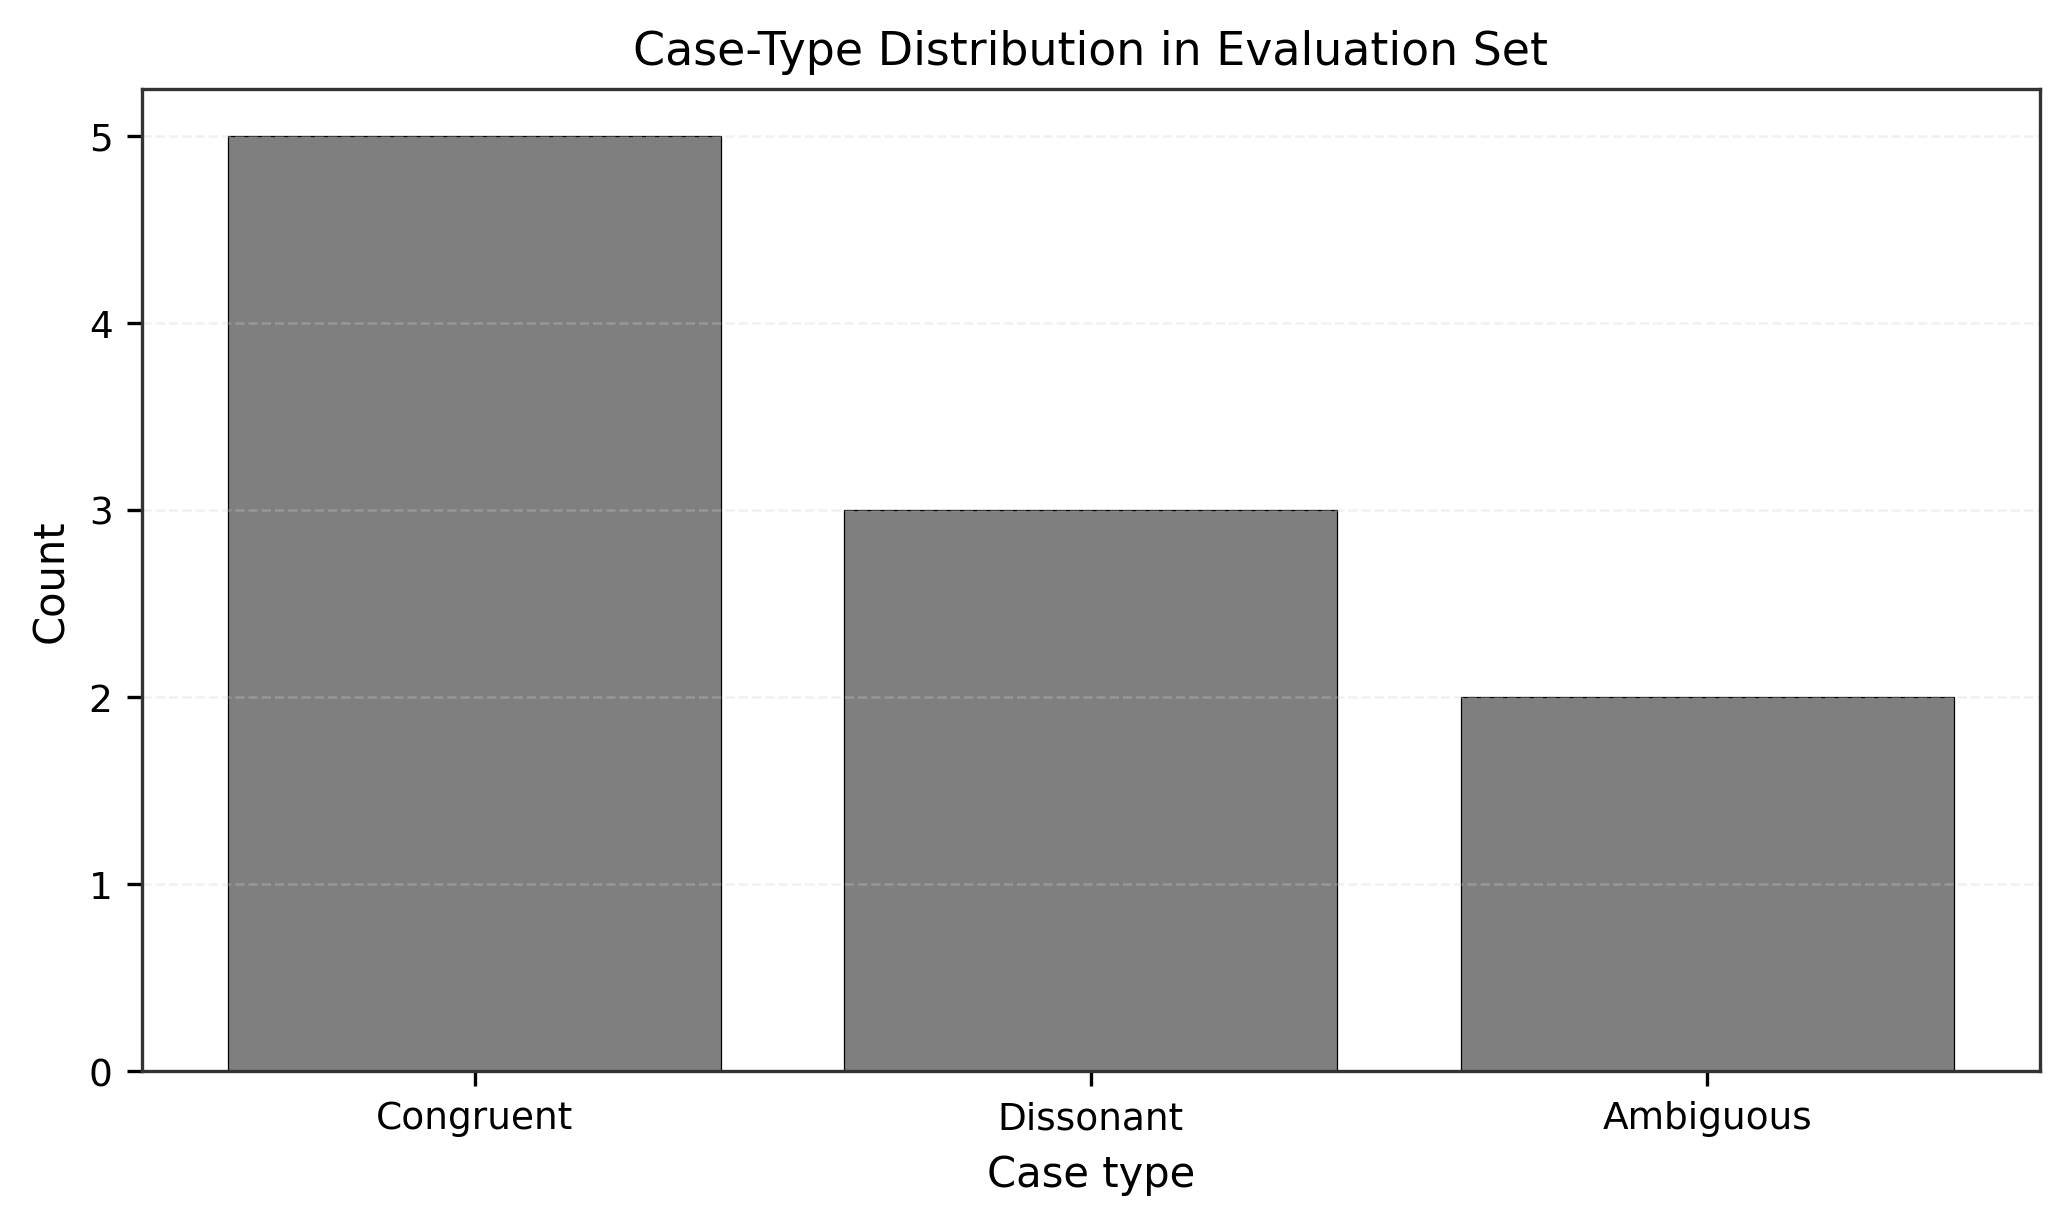
\includegraphics[width=\linewidth]{figures/case_type_distribution_plot.png}
    \caption{Distribution of congruent, dissonant, and ambiguous cases used in evaluation.}
    \label{fig:case_type_distribution_plot}
\end{figure}

% Table inclusion options:
% Option A: include all generated table environments.
% Auto-generated paper tables for IEEE-style insertion
\begin{table*}[t]
\centering
\footnotesize
\caption{System components and implementation mapping for the bimodal affective alignment prototype.}
\label{tab:system_components}
\begin{tabular}{|p{0.18\linewidth}|p{0.20\linewidth}|p{0.27\linewidth}|p{0.27\linewidth}|}
\hline
Component & Implementation & Role & Robustness/Notes \\
\hline
Text Emotion Module & app/text\_emotion.py & Infers emotion probabilities from user text. & Rule-based lexical scoring; stable for classroom demo, limited linguistic nuance. \\
Face Emotion Module & app/face\_emotion.py & Extracts facial emotion probabilities from image input. & Includes safe fallback profile when image/face signal is weak. \\
Fusion Module & app/fusion.py & Combines modality probabilities with weighted alpha fusion. & Normalized combination reduces single-modality dominance. \\
Response Generator & app/response\_generator.py & Generates empathetic response conditioned on detected emotion. & Uses deterministic templates for reproducible output. \\
Evaluation Module & app/final\_evaluation\_pack.py + app/plot\_results.py & Builds rating sheets, aggregates metrics, and outputs figures/tables. & Supports pilot human study and reproducible CSV/plot generation. \\
\hline
\end{tabular}
\end{table*}

\begin{table*}[t]
\centering
\footnotesize
\caption{Mode-level comparison used in the course project evaluation design.}
\label{tab:mode_comparison}
\begin{tabular}{|p{0.12\linewidth}|p{0.12\linewidth}|p{0.21\linewidth}|p{0.21\linewidth}|p{0.24\linewidth}|}
\hline
Mode & Input & Strength & Limitation & Expected Use \\
\hline
Text-only & User text & Captures explicit semantic and affective wording. & Cannot use facial context; may miss non-verbal cues. & Text-rich interactions, chat logs, and typed feedback. \\
Face-only & Facial image & Uses non-verbal affective cues independent of wording. & Sensitive to image quality and expression ambiguity. & Vision-available settings where text is unavailable. \\
Fused bimodal & Text + facial image & Integrates complementary cues and improves robustness. & Requires both modalities and tuning of alpha. & Primary mode for balanced affect-aware responses. \\
\hline
\end{tabular}
\end{table*}

% Preliminary human evaluation (pilot) with one completed rater (R1).
\begin{table*}[t]
\centering
\footnotesize
\caption{Preliminary human evaluation summary across modes (pilot, one completed rater R1).}
\label{tab:human_eval_pilot}
\begin{tabular}{|p{0.12\linewidth}|p{0.12\linewidth}|p{0.21\linewidth}|p{0.21\linewidth}|p{0.24\linewidth}|}
\hline
Mode & Empathy & Social Presence & Trust & Helpfulness \\
\hline
Text only & 3.4 & 3.1 & 4.0 & 3.5 \\
Face only & 2.7 & 2.3 & 3.0 & 2.7 \\
Fused & 4.5 & 4.2 & 4.6 & 4.6 \\
\hline
\end{tabular}
\end{table*}

\begin{table*}[t]
\centering
\footnotesize
\caption{Representative dissonant cases from the implemented case-study set.}
\label{tab:dissonance_cases}
\begin{tabular}{|p{0.22\linewidth}|p{0.09\linewidth}|p{0.09\linewidth}|p{0.10\linewidth}|p{0.33\linewidth}|p{0.09\linewidth}|}
\hline
User Text & Text Emotion & Face Emotion & Fused Emotion & Response & Case Type \\
\hline
I am thrilled with the result, even though the atmosphere around me feels gloomy. & happy & sad & happy & I am happy with the result. & Dissonant \\
I feel sad and drained after losing the opportunity, even though the people around me seem upbeat. & sad & happy & sad & I feel sad and drained after losing the opportunity. & Dissonant \\
I am frustrated about the delay, even though everything around me feels calm. & angry & neutral & neutral & I am frustrated about the delay. & Dissonant \\
\hline
\end{tabular}
\end{table*}

\begin{table*}[t]
\centering
\footnotesize
\caption{Alpha-sensitivity summary from the implemented fusion sweep.}
\label{tab:alpha_sensitivity_summary}
\begin{tabular}{|p{0.12\linewidth}|p{0.12\linewidth}|p{0.21\linewidth}|p{0.21\linewidth}|p{0.24\linewidth}|}
\hline
Alpha & Dominant Fused Emotion & Text-Match Rate & Face-Match Rate & Neutral Share \\
\hline
0.0 & neutral & 0.25 & 1.0 & 1.0 \\
0.25 & neutral & 0.25 & 1.0 & 1.0 \\
0.5 & neutral & 0.25 & 1.0 & 1.0 \\
0.75 & neutral & 0.5 & 0.75 & 0.75 \\
1.0 & neutral & 1.0 & 0.25 & 0.25 \\
\hline
\end{tabular}
\end{table*}


% Option B: copy individual tables from docs/paper_assets/tables/*.md or *.csv into custom IEEE layouts.
